\section{Lecture 12: Low Power Architecture}
For some applications, low power consumption is more important than performance:
\begin{itemize}
\item Mobile communication and computing
\item Wirteless internet
\item Medical implants
\item Deep space applications 
\end{itemize}

Low-power designs will lead to:
\begin{itemize}
\item Longer battery life time
\item Lower cost (Cooling and package, Electricity bill)
\item Higher reliability and longer life time (due to lower temperature and smaller temperature gradients).
  \newline
\end{itemize}

\begin{figure}[H]
  \centering
  \scalebox{0.5}{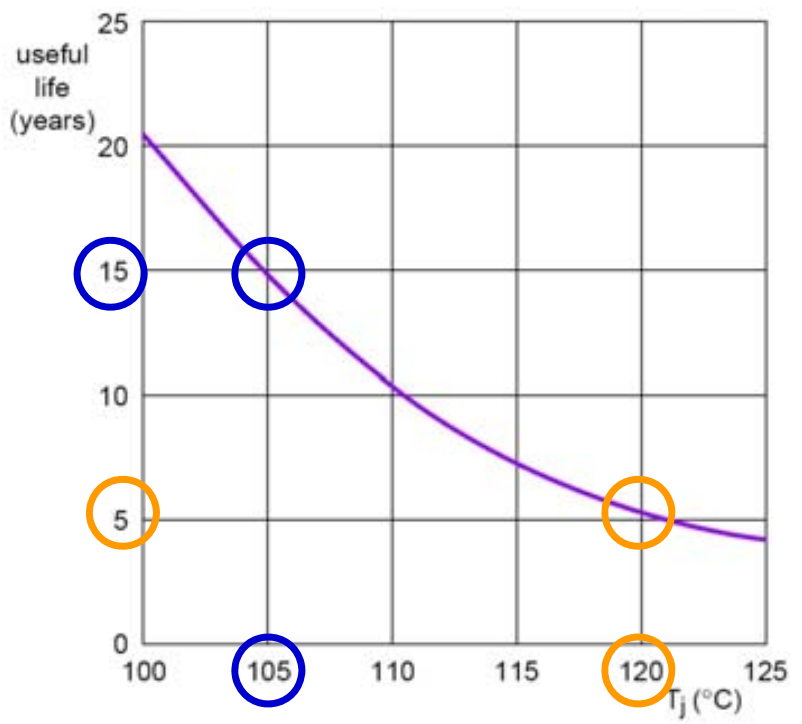
\includegraphics{img/thermal-reliability.png}}
  \caption{How the temperature affects the lifespan of a processor.}
  \label{fig:thermal-reliability}
\end{figure}

\subsection{Low-Power Techniques}
What can we do to reduce power consumption. At a low level we can use sign-magnitude representation over two complements representation for integer, this is because when using twos complement and switching between positive and negative numbers, almost all bits needs to be switched as can be seen in figure \ref{fig:2comp-vs-sign}

\begin{figure}[H]
  \centering
  \scalebox{0.5}{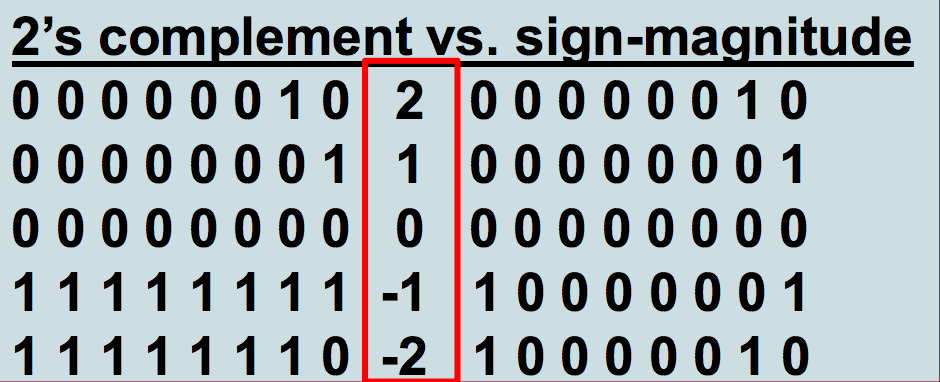
\includegraphics{img/2comp-vs-sign.png}}
  \caption{two's complement vs sign-magnitude representation.}
  \label{fig:2comp-vs-sign}
\end{figure}

We can also optimize with software such as:
\begin{itemize}
\item Use power efficient algorithms.
\item Compiler to optimize for more power efficient code.
\item Run-time power management by the OS.
\end{itemize}


\subsection{Design for low power \todo{kanske kan plocka bort denna och låta allt stå under första rubriken}}
\subsection{The Cursoe Processors}
\subsection{The ARM Processors}
\subsection{Final remarks}
